\chapter{Tecnologie e strumenti utilizzati}\label{cap:Tecnologie e strumenti utilizzati}
Per il raggiungimento degli obiettivi del progetto di stage sono state utilizzate diverse tecnologie e strumenti. 
In questa sezione verranno riepilogate con una breve descrizione del loro utilizzo. 
\section{Linguaggi utilizzati}
\subsection{YAML}
YAML, acronimo di YAML Ain't Markup Language, è un linguaggio di Markup, noto per la sua leggibilità e la sua 
chiarezza espressiva. \\
La prima idea attorno al linguaggio YAML nasce attorno agli anni '90 quando Clark C. Evans, software developer, lo propone come alternativa a XML.\\
Nel 2001 Evans pubblica la prima specifica del linguaggio, che va a definire i principi fondamentali del linguaggio.\\
Negli anni YAML ha acquisito sempre più popolarità e interesse di utilizzo, in quanto ha offerto una configurazione semplice e leggibile 
per strumenti si DEVOPS, orchestrazione, automazione e molto altro (Figura \ref{fig:yaml}).\\
La storia di YAML è strettamente legata alla esigenza di semplificare la rappresentazione di dati complessi, 
in un formato più comprensibile a un essere umano e a macchine.\\
\begin{figure}[hpp]
    \centering
    
\includegraphics[width=0.5\textwidth]{images/tecnologie/logo_yaml.png}
    \caption{Logo di YAML}
    \label{fig:yaml}
\end{figure}
\pagebreak
\subsection{Python}
Python è un linguaggio di programmazione ad alto livello, orientato agli oggetti,
che si distingue per la sua sintassi chiara e intuitiva (Figura \ref{fig:python}).\\
Creato da Guido van Rossum e rilasciato per la prima volta nel 1991, è cresciuto fino a 
diventare uno dei linguaggi più utilizzati al mondo.\\
Data la sua semplicità e la sua versatilità, Python è utilizzato in diversi ambiti dallo sviluppo web, alla \gls{Data Analytics}{}, allo sviluppo di applicazione 
desktop e mobile, fino ad arrivare all'automazione e all'intelligenza artificiale.\\
\begin{figure}[hpp]
    \centering
    
\includegraphics[width=0.5\textwidth]{images/tecnologie/logo_python.png}
    \caption{Logo di Python}
    \label{fig:python}
\end{figure}
\section{Tecnologie utilizzate}

\subsection{Metodologia di sviluppo e strumenti di gestione di progetto}
\subsubsection{Click Up}   %strumento di issue tracking system utilizzato


\subsection{Ambiente di sviluppo}
\subsubsection{Docker Compose}

\subsection{Versioning}
\subsubsection{Git}
\textbf{Git} è un sistema di controllo versione distribuito, utilizzato per il tracciamento delle modifiche ai file di un progetto.\\ 
Creato da Linus Torvalds nel 2005, GIT è stato pensato per la gestione del codice sorgente del kernel Linux, ma è stato adottato 
per progetti di ogni genere, di piccole e grandi dimensioni (Figura \ref{fig:git}).\\
\begin{figure}[hpp]
    \centering
    
\includegraphics[width=0.4\textwidth]{images/tecnologie/logo_git.png}
    \caption{Logo di Git}
    \label{fig:git}
\end{figure}

\noindent È uno dei sistemi di controllo di versione più utilizzati al mondo, grazie alla sua velocità, alla sua efficienza e alla sua flessibilità.\\
Come tutti i sistema di controllo di versione si basa sul concetto di \gls{repository}{}, ovvero un archivio contenente i file e tutti i 
\gls{metadati}{} relativi alle modifiche effettuate.\\  
In \textbf{Git} un file può trovarsi in tre stati diversi: \textit{commited} (versionati), \textit{modified} (modificati) e \textit{staged} (pronti per essere versionati).\\
Ogni nuovo modifica, se versionata all'interno del \gls{repository} viene identificata da un \textit{commit}, avente un identificativo univoco di 40 caratteri. Modificato 
significa che il file è stato modificato ma non è ancora stato versionato, mentre staged significa che il file è stato modificato e preparato per essere inserito nel 
prossimo \textit{commit}.\\
Quanto detto illustra le operazioni essenziali che possono essere effettuate con \textbf{Git} (Figura \ref{fig:git_workflow}).
\begin{figure}[hpp]
    \centering
    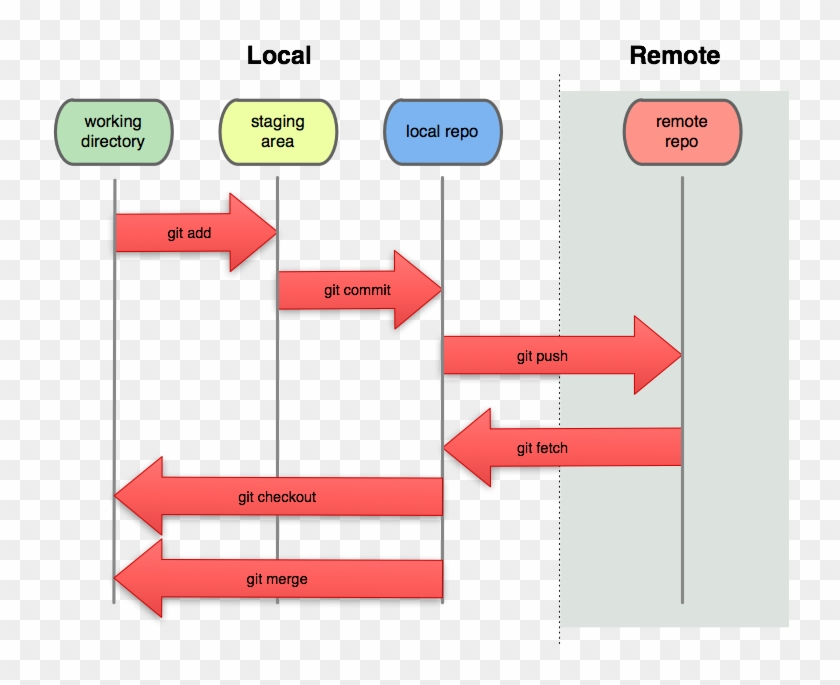
\includegraphics[width=0.5\textwidth]{images/tecnologie/comandi_git.png}
    \caption{Comandi di base di Git}
    \label{fig:git_workflow}
\end{figure}
Essenzialmente un workflow di bse con \textbf{Git} prevede:
\begin{list}{-}{}
    \item \textbf{Clonare} un \gls{repository}{}, se già esistente;
    \item \textbf{Modificare} i file all'interno della \gls{working directory}{};
    \item \textbf{Stage} dei file, ovvero prepararli per il prossimo \textit{commit}, aggiungendoli alla \textit{staging area} con il comando \textit{git add};
    \item \textbf{Commit} dei file, ovvero versionarli, con il comando \textit{git commit}, i file così come son salvati nella \textit{staging area} vengono versionati all'interno del \gls{repository}{};
    \item \textbf{Push} delle modifiche sul \gls{repository}{} remoto.
\end{list}
\pagebreak
\subsubsection{GitHub}
Per quanto riguarda il servizio di hosting che ha ospita il \gls{repository}{} remoto è stato utilizzato \textbf{GitHub}, andando a condividere 
i contenuti tra il mio account e quello del tutor aziendale (Figura \ref{fig:github}).\\
\begin{figure}[hpp]
    \centering
    
\includegraphics[width=0.4\textwidth]{images/tecnologie/logo_github.png}
    \caption{Logo di GitHub}
    \label{fig:github}
\end{figure}
\\
GitHub è una piattaforma di hosting per progetti software, che utilizza \textbf{Git} come sistema di controllo di versione e contiene tutti 
i file e i \gls{metadati}{} relativi alle modifiche validate lungo le fasi del progetto.\\
\subsection{Documentazione}